\documentclass[10pt]{beamer}
\usepackage[T1]{fontenc}
\usepackage[utf8]{inputenc}
\usepackage[slovene]{babel}
\usepackage{pgfpages} % privat zapiski
\usepackage{amsmath} % pravilen izpis v "math mode"
\usepackage{hyperref}
\usepackage{pgfplots}
\usepackage{tikz}
\usepackage{algorithm}
\usepackage{algorithmicx}

%\usepackage{biblatex}
%\addbibresource{literatura}

\usepackage{algpseudocode}
%\documentclass{standalone}
%\usepackage{pgfplotstable,filecontents}
\usepackage{bibentry}

\usepackage{caption}

\DeclareCaptionFormat{myformat}{#3}
\captionsetup[algorithm]{format = myformat}

\pgfplotsset{compat=1.8}
\hypersetup{hidelinks}
%\usetheme{Bergen}
\usecolortheme{seahorse}

\usepackage{graphicx}% http://ctan.org/pkg/graphicx
\usepackage{booktabs}% http://ctan.org/pkg/booktabs

\usepackage{palatino}
\usefonttheme{serif}
\DeclareMathOperator{\logit}{logit}
\setbeamertemplate{navigation symbols}{} % izklop navigacije
\setbeamertemplate{footline}[frame number]{} % oštevilčenje
\setbeamertemplate{note page}{\pagecolor{yellow!5}\insertnote}
\setbeamertemplate{itemize items}[circle]



\begin{document}
    \title[Diplomski seminar]{Iterativne numerične metode v posplošenih linearnih modelih}
    \author{Mitja Mandić \\ \small Mentor: izr. prof. dr. Jaka Smrekar}
    \date{9. september 2021}

\begin{frame}
    \titlepage
\end{frame}

\begin{frame}{Eksponentna družina}
    \begin{itemize}
        \item<1->Porazdelitev pripada enoparametrični eksponentni družini z disperzijskim parametrom, če
        ima gostoto oblike
            \begin{equation*}
            f_{Y}(y; \theta, \phi) = \exp{\left(\frac{y\theta - b(\theta)}{a(\phi)} + c(y, \phi)\right)},
        \end{equation*}
        $\theta$ imenujemo \textit{naravni} ali \textit{kanonični} parameter, $\phi$ pa \textit{disperzijski} parameter
        \pause
        \item Velja $\mathbb{E}(Y) = b'(\theta)$ in $\mathrm{Var}(Y) = b''(\theta)a(\phi)$\pause
        \item Za $Y\sim N(\mu,\sigma^2)$ z gostoto $\tfrac{1}{\sqrt{2\pi\sigma^2}}\exp{(-\tfrac{(y-\mu)^2}{2\sigma^2})}$
         izrazimo
        \[
            \theta = \mu,~\phi = \sigma^2,~a(\sigma^2)=\sigma^2,~b(\mu) = \frac{\mu^2}{2}
        \] \pause
        \item Za $Y\sim Bin(m,p)$ je $\mathrm{P}(Y = y) = \binom{m}{y}p^y(1-p)^{m-y},$ kar preoblikujemo v        \[
        \exp\left(y\log\left(\frac{p}{1-p}\right) + m\log(1-p) + \log{\binom{m}{y}}\right)
        \] in preberemo $\theta = \log\frac{p}{1-p},~b(\theta) = m\log(1 + e^{\theta}),~a(\phi) = 1.$
    \end{itemize}
\end{frame}


\begin{frame}{Posplošeni linearni modeli}    
Vsak posplošeni linearni model sestavljajo trije deli:
\begin{itemize}
    \item \alert{slučajni del} -- porazdelitev proučevane slučajne spremenljivke \pause
    \item \alert{sistematični del} -- linearna relacija med pojasnjevalnimi spremenljivkami \pause
    \item \alert{povezovalna funkcija} -- povezava med sistematičnim delom in pričakovano vrednostjo. Če je enaka naravnemu parametru
    porazdelitve ji rečemo \textit{kanonična} povezovalna funkcjia \pause
\end{itemize}
Skupaj:
\[
    g(\mu) = X\beta
\]
\end{frame}

\begin{frame}[t]
    \frametitle{Logistični model}
    
        \begin{itemize}
            \item<1-> Predpostavimo binomsko porazdelitev $Y$. Uporablja se za računanje verjetnosti iz binarnih podatkov, model je oblike
            \[
                \logit(p) = \log\left(\frac{p}{1-p}\right) = X\beta
            \]
            \item<2->Izrazimo 
            \[
                p_{i} = \frac{\exp(x_{i}^\top\beta)}{1 + \exp(x_{i}^\top\beta)}
            \]
            \pause
            \only<2>{
            \begin{figure}
                \includegraphics[width=5cm]{sigmoida.png}
            \end{figure}
            }
            \item<3-> Logaritemska funkcija verjetja, funkcija zbira in njen odvod
            \begin{align*}
                \ell(\beta) &= \sum_{i=1}^{n}\left( y_{i}(x_{i}^\top\beta) - m_{i}\log(1 + \exp({x_{i}^\top\beta}))\right)\\
                \frac{\partial}{\partial\beta_{j}}\ell(\beta)&=\sum_{i=1}^{n} \left(x_{ij}(y_{i} - \mu_{i})\right),~~j=0,\ldots,r\\
                \frac{\partial^2}{\partial\beta_{j}\partial\beta_{k}}\ell(\beta) &= -\sum_{i=1}^{n}\left(x_{ij}v_{i}(\beta)x_{ik}\right),~~j,k=0,\ldots,r
            \end{align*}

            \end{itemize}
\end{frame}
\begin{frame}\frametitle{Probit model}
    \[
        p = \Phi(X\beta)
    \]
    \begin{itemize}
            \item Razvit v enake namene kot logistični model, znova se za $Y$ predpostavi binomsko porazdelitev
            \item Vidimo, da povezovalna funkcija $\Phi^{-1}(p)$ \underline{ni} kanonična
            \pause
            \item Logaritemska funkcija verjetja, funkcija zbira in njen odvod
            \begin{align*}
                \ell(\beta) &= \sum_{i = 1}^{n}\left(y_{i}\log\Phi(x_{i}^\top\beta) + (m_{i} - y_{i})\log(1 - \Phi(x_{i}^\top\beta)) \right) \\
                \frac{\partial}{\partial\beta_{j}}\ell(\beta) &= \sum_{i=1}^{n}\frac{y-m_{i}\Phi(x_{i}^\top\beta)}{\Phi(x_{i}^\top\beta)(1-\Phi(x_{i}^\top\beta))}
                \phi(x_{i}^\top\beta)x_{ij},~~j=0,\ldots,r \\
                \begin{split}
                    \frac{\partial^2}{\partial\beta_{j}\partial\beta_{k}}\ell(\beta) &= \sum_{i = 1}^{n}
                    x_{ij}\frac{(y_{i}-m_{i}\Phi(x_{i}^\top\beta))(-\phi(x_{i}^\top\beta)x_{i}^\top\beta) - m_{i}\phi(x_{i}^\top\beta)^2}{\Phi(x_{i}^\top\beta)(1-\Phi(x_{i}^\top\beta))}x_{ik} - \\
                    &-x_{ij}\frac{\phi(x_{i}^\top\beta)^2(1-2\Phi(x_{i}^\top\beta))}{(\Phi(x_{i}^\top\beta)(1-\Phi(x_{i}^\top\beta)))^2}x_{ik},~~j,k=0,\ldots,r
                \end{split}
            \end{align*}
    \end{itemize}

\end{frame}

\begin{frame}{Metoda največjega verjetja}
    \begin{itemize}
        \item Najprej privzemimo gostote oblike $f_{X}(x;\theta) = f(x;\theta_{1},\ldots,\theta_{r})$ za nek $\theta \in \Theta^{r}$
        
        \item Pri fiksni realizaciji poskusa definiramo \textit{funkcijo verjetja}
        \[ 
            F(X_{1},\ldots,X_{n};\underbrace{\theta_{1},\ldots,\theta_{r}}_{\theta}) = f(X_{1},\theta)\cdots f(X_{n},\theta) 
        \] 
        \item Iščemo njen maksimum, kar bo hkrati tudi maksimum $\log(F)$
        \pause
        \item Sistemu 
        \[
            \frac{\partial}{\partial \theta_{j}}\log F (X,\theta) = 0,~~j=1,\ldots,r
        \]
        pravimo sistem enačb verjetja, njegova rešitev je kandidatka za \textit{cenilko največjega verjetja}
        \pause
        \item Niso nujno nepristranske, so pa dosledne, če je rešitev enolična
        \item \textbf{Običajno niso eksplicitno rešljive}
    \end{itemize}
\end{frame}

\begin{frame}[t]
    \frametitle{Obstoj cenilke največjega verjetja v logističnem modelu}
\begin{columns}
    \begin{column}{5cm}
\only<1->{
        \begin{center}
            \begin{figure}[h!]
            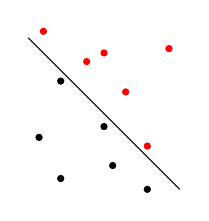
\begin{tikzpicture}[scale = 0.55, transform shape]
            %\draw (0,4) -- (0,0) -- (4,0);
            \draw (3.75,0.25) -- (0.25,3.75);
            \filldraw[black] (2.2,0.8) circle (2pt);
            \filldraw[black] (1,2.75) circle (2pt);
            \filldraw[black] (2,1.7) circle (2pt);
            \filldraw[black] (0.5,1.45) circle (2pt);
            \filldraw[black] (1,0.5) circle (2pt);
            \filldraw[black] (3,0.25) circle (2pt);
            
            \filldraw[red] (3,1.25) circle (2pt);
            \filldraw[red] (2,3.4) circle (2pt);
            \filldraw[red] (1.6,3.2) circle (2pt);
            \filldraw[red] (3.5,3.5) circle (2pt);
            \filldraw[red] (0.6,3.9) circle (2pt);
            \filldraw[red] (2.5,2.5) circle (2pt);
            
            \end{tikzpicture}
            \caption{Popolna separacija. Rešitev ne obstaja}
        \end{figure}
        \end{center}
}
\only<2->{
        \begin{center}
            \begin{figure}%[h!]
            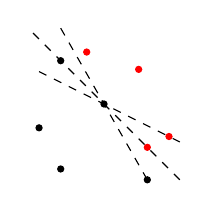
\begin{tikzpicture}[scale = 0.55, transform shape]
            %\draw (0,4) -- (0,0) -- (4,0);
            \draw[dashed] (3.75,0.25) -- (0.25,3.75);
            \draw[dashed] (1,3.75) -- (3,0.25);
            \draw[dashed] (0.5,2.75) -- (3.75,1.125);
        
            %\filldraw[black] (2.2,0.8) circle (2pt);
            \filldraw[black] (1,3) circle (2pt);
            \filldraw[black] (2,2) circle (2pt);
            \filldraw[black] (0.5,1.45) circle (2pt);
            \filldraw[black] (1,0.5) circle (2pt);
            \filldraw[black] (3,0.25) circle (2pt);
            
            \filldraw[red] (3,1) circle (2pt);
            \filldraw[red] (1.6,3.2) circle (2pt);
            \filldraw[red] (3.5,1.25) circle (2pt);
            \filldraw[red] (2.8,2.8) circle (2pt);
            
            \end{tikzpicture}
            \caption{Nepopolna separacija, drugi primer. Rešitev ne obstaja}
            \label{fig:neenolicna}
        \end{figure}
        \end{center}
}
    \end{column}

    \begin{column}{5cm}
        \only<2->{
        \begin{center}
            \begin{figure}[t!]
            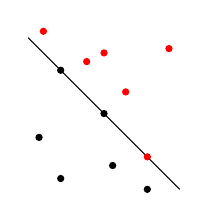
\begin{tikzpicture}[scale = 0.55, transform shape]
            %\draw (0,4) -- (0,0) -- (4,0);
            \draw (3.75,0.25) -- (0.25,3.75);
            \filldraw[black] (2.2,0.8) circle (2pt);
            \filldraw[black] (1,3) circle (2pt);
            \filldraw[black] (2,2) circle (2pt);
            \filldraw[black] (0.5,1.45) circle (2pt);
            \filldraw[black] (1,0.5) circle (2pt);
            \filldraw[black] (3,0.25) circle (2pt);
            
            \filldraw[red] (3,1) circle (2pt);
            \filldraw[red] (2,3.4) circle (2pt);
            \filldraw[red] (1.6,3.2) circle (2pt);
            \filldraw[red] (3.5,3.5) circle (2pt);
            \filldraw[red] (0.6,3.9) circle (2pt);
            \filldraw[red] (2.5,2.5) circle (2pt);
            
            \end{tikzpicture}
            \caption{Nepopolna separacija, prvi primer. Rešitev ne obstaja}
            \label{fig:enolicna}
        \end{figure}
        \end{center}
        }
        \only<3>{
        \begin{center}
            \begin{figure}[h!]
            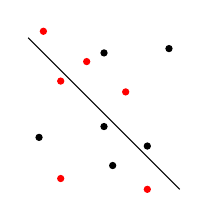
\begin{tikzpicture}[scale = 0.55, transform shape]
            %\draw (0,4) -- (0,0) -- (4,0);
            \draw (3.75,0.25) -- (0.25,3.75);
            \filldraw[black] (2.2,0.8) circle (2pt);
            \filldraw[red] (1,2.75) circle (2pt);
            \filldraw[black] (2,1.7) circle (2pt);
            \filldraw[black] (0.5,1.45) circle (2pt);
            \filldraw[red] (1,0.5) circle (2pt);
            \filldraw[red] (3,0.25) circle (2pt);
            
            \filldraw[black] (3,1.25) circle (2pt);
            \filldraw[black] (2,3.4) circle (2pt);
            \filldraw[red] (1.6,3.2) circle (2pt);
            \filldraw[black] (3.5,3.5) circle (2pt);
            \filldraw[red] (0.6,3.9) circle (2pt);
            \filldraw[red] (2.5,2.5) circle (2pt);
            
            \end{tikzpicture}
            \caption{Prekrivanje. Rešitev obstaja in je enolična}
        \end{figure}
        \end{center}
        }
    \end{column}
\end{columns}
\end{frame}

\begin{frame}{Numerične metode}
    \begin{itemize}
        \item
        Iterativne metode, ki temeljijo na Newtonovi metodi za iskanje ničel funkcije
        \[
            x_{i+1} = x_{i} - \frac{f(x_{i})}{f'(x_{i})}
        \]
        \pause
        \item Za iskanje \underline{ekstremov} logaritemske funkcije verjetja metodo prilagodimo.
        Enačimo gradient $\ell(\theta)$ z nič in dobimo
        \[
            \theta_{i+1} = \theta_{i} - \left(\frac{\partial^2}{\partial\theta^2}\ell(\theta_{i})\right)^{-1}\frac{\partial}{\partial\theta}\ell(\theta_{i}).
        \]
        Računanje in invertiranje Hessiana pa je lahko problematično. Kako se temu izognemo?
        \pause
        \item Namesto inverza uvedemo računanje premikov. Iteracijski korak je tako
        \begin{align*}
            \left(\frac{\partial^2}{\partial\theta^2}\ell(\theta_{i})\right) h &= -\frac{\partial}{\partial\theta}\ell(\theta_{i}) \\
            \theta_{i+1} &= \theta_{i} + h
        \end{align*}
        
    \end{itemize}
    
\end{frame}

\begin{frame}{Fisherjeva zbirna metoda}

\[
    \theta_{i+1} = \theta_{i} + \mathrm{FI}(\theta_{i})^{-1}\left(\frac{\partial}{\partial\theta}\ell(\theta_{i})\right),
\]
kjer je $\mathrm{FI}(\theta) = \mathbb{E}\left((\frac{\partial}{\partial\theta}\ell)(\frac{\partial}{\partial\theta}\ell)^\top\right).$
\pause
\textit{Informacijska enakost} pravi
\begin{equation*}
    \mathrm{FI}(\theta) = \mathbb{E}\left((\frac{\partial}{\partial\theta} \ell)(\frac{\partial}{\partial\theta} \ell)^\top\right) = -\mathbb{E}\left(\frac{\partial^2}{\partial\theta^2}\ell\right),
\end{equation*}
\pause
V nalogi smo za \underline{kanonične povezovalne funkcije} dokazali
\[
    \mathbb{E}\left(\frac{\partial^2}{\partial\theta^2}\ell\right) = \frac{\partial^2}{\partial\theta^2}\ell
\]
in sledi
\[
    \mathrm{FI}(\theta) = -\frac{\partial^2}{\partial\theta^2}\ell
\]
\pause
$\rightarrow$ za kanonične povezovalne funkcije Fisherjeva zbirna metoda in Newtonov algoritem sovpadata!
\end{frame}

\begin{frame}{Fisherjeva zbirna metoda}
Velja še:
\[
    -\frac{\partial^2}{\partial\theta^2}\ell = \mathrm{FI}(\theta) = \mathrm{Var}\left(\frac{\partial}{\partial\theta}\ell\right),
\]
torej je Hessejeva matrika log-verjetja negativno semidefinitna.
\pause
Taylorjev polinom za funkcijo zbira (ob upoštevanju $\frac{\partial}{\partial\theta}\ell(\theta^{*}) = 0$) je
\[
    \ell(\theta^{*} + s) = \ell(\theta^{*}) + \frac{1}{2}s^\top \frac{\partial^2}{\partial\theta^2}\ell(\theta^{*})s.
\]
\pause
\begin{enumerate}[$\Rightarrow$]
    \item imamo konveksen optimizacijski problem
    \item reševanje sistema enačb za premik je enostavnejše 
\end{enumerate}
\end{frame}

%\begin{frame}
%    \frametitle{Iteracijski korak logističnega modela}
%    \begin{itemize}
%        \item \textbf{Logistični model}
%        \begin{itemize}
%            \item<1->
%            Iteracijski korak v logistični regresiji smo izpeljali kot
%            \begin{align*}
%                \underbrace{(X^\top v(\hat{\beta}_{i}) X)}_{\text{Fisher info}}h &= \underbrace{X^\top(y - \mu(\hat{\beta}_{i}))}_{\text{funkcija~zbira}} \\
%                    \hat{\beta}_{i+1} &= \hat{\beta}_{i} + h
%            \end{align*}
%        \end{itemize}
%
%\end{itemize}
%\end{frame}
\begin{frame}[shrink]%[allowframebreaks]
\begin{center}
    \only<1>{
        Iteracijski korak logističnega modela:
        \begin{align*}
            \underbrace{(X^\top v(\hat{\beta}_{i}) X)}_{\text{Fisher info}}h &= \underbrace{X^\top(y - \mu(\hat{\beta}_{i}))}_{\text{funkcija~zbira}} \\
            \hat{\beta}_{i+1} &= \hat{\beta}_{i} + h
        \end{align*}
        }    
        \only<2->{
        \begin{minipage}{0.7\linewidth}
        \begin{center}
    %\scalebox{0.75}{
        
        
    \begin{algorithm}[H]
    \caption{\textbf{function} oceniParametre(iteracije, X, Y, $\beta_{zacetni}$, $\epsilon$)}
    \begin{algorithmic}
        \State $p = \frac{\exp{(X^\top \beta_{star})}}{1 + \exp{(X^\top \beta_{star})}}$
        \State $V = p(1 - p)$ 
        \State $Score = X^\top (Y - p)$ 
        \State $Info = X^\top V X$ 
        \State \text{\textit{\textbf{Reši sistem na h:}}} $Info * h = Score$
        \State $\beta_{star} = \beta_{zacetni}$
        \State $\beta_{nov} = \beta_{star} + h$
        \While{$i \leq iteracije$}
        %\framebreak
            \If{$\beta_{nov} - \beta_{star} \geq \epsilon$}
                \State $p = \frac{\exp{(X^\top \beta_{nov})}}{1 + \exp{(X^\top \beta_{nov})}}$ 
                \State $V = p(1 - p)$ 
                \State $Score = X^\top (Y - p)$ 
                \State $Info = X^\top V X$ 
                \State \text{\textit{\textbf{Razreši na h:}}} $Info * h = Score$ 
                \State $\beta_{star} = \beta_{nov}$ 
                \State $\beta_{nov} = \beta_{star} + h$ 
            \Else
            
            \State \text{\textit{Dosegli smo želeno natančnost v zadostnem številu korakov}}
            \Return $\beta_{nov}$
            
            \EndIf
            
        \EndWhile
    \end{algorithmic}
\end{algorithm}

\end{center}
\end{minipage}
}
\end{center}
\end{frame}

%
\begin{frame}[t]
    \frametitle{Rezultati}
    Iz interneta smo pridobili podatke o odpovedi tesnil iz vesoljskih poletov pred dobo \textit{Challengerja}
    in izračunali:
\begin{columns}
    \begin{column}{6.5cm}
    \begin{itemize}
        \item<1-> verjetnost odpovedi z logistično regresijo le s podatki o temperaturi
        \item<2-> verjetnost odpovedi s temperaturo in pritiskom
        \item<3> primerjava logistične in probit regresije le s podatki o temperaturi
    \end{itemize}
\end{column}
\begin{column}{5.5cm}
\only<1>{
    \begin{figure}
    \includegraphics[width=5.5cm]{logit_challenger.jpeg}
\end{figure}
}
\only<2>{
    \begin{figure}
        \includegraphics[width=5.5cm]{logit_3d.png}
    \end{figure}
}
\only<3>{
    \begin{figure}
        \includegraphics[width=5.5cm]{logit_probit.png}
    \end{figure}
}
\end{column}
\end{columns}
\end{frame}

\begin{frame}
    \frametitle{Povzetek}
    \begin{itemize}
        \item Želeli smo bolje razumeti ozadje računanja parametrov v posplošenih linearnih modelih
        \item Za logistični model smo izpeljali enačbe verjetja in raziskali kdaj rešitve obstajajo
        \item Formule smo posplošili za vse modele s porazdelitvami iz eksponentne družine in videli prednosti uporabe kanoničnih povezovalnih funkcij
        \item Newtonovo metodo smo prilagodili za iskanje ekstremov in dokazali njeno sovpadanje z Fisherjevo zbirno metodo za kanonične modele
        \item Vso teorijo smo na koncu povezali v praktičnih primerih
    \end{itemize}
\end{frame}

\begin{frame}[t, allowframebreaks]
    \frametitle{Literatura}
    \nocite{*}
    \bibliographystyle{abbrv}
    \bibliography{literatura}
\end{frame}

\end{document}